\begin{appendix} %Anhang
\section{Anhang}

\includepdf[pages=2, scale=0.8, angle=0, pagecommand={
\subsection{Aufgabenstellung im Originalwortlaut}
\label{aufgabenstellung_originalwortlaut}}]
{11_PDFs/fhnw_pro6m_alexandrit_femtosekunden_laser_disposition_rev_4.pdf}

\includepdf[pages=3, scale=0.8, angle=0, pagecommand={
% \subsection{Aufgabenstellung im Originalwortlaut}
\label{aufgabenstellung_originalwortlaut}}]
{11_PDFs/fhnw_pro6m_alexandrit_femtosekunden_laser_disposition_rev_4.pdf}

\includepdf[pages=4, scale=0.8, angle=0, pagecommand={
% \subsection{Aufgabenstellung im Originalwortlaut}
\label{aufgabenstellung_originalwortlaut}}]
{11_PDFs/fhnw_pro6m_alexandrit_femtosekunden_laser_disposition_rev_4.pdf}

\subsection{Stückliste der Verwendeten Materialien}
\begin{table}[H]
    \centering
    \begin{tabular}{c|l|l}
        Stückzahl& \textbf{Bauteil}&       \textbf{Beschreibung}\\
        \hline
        1&          TEC-Treiber&           TEC 1122 - Meerstetter Engineering GmbH\\
        1&          Diodentreiber&         LPLDD-1,5A-35V-TP-H - Optlasers.com\\
        1&          Laserdiode&            K635EWDFN-5.000W - bwt-bj.com\\
        1&          Raspberry PI&          Raspberry PI 3B+\\
        1&          Betriebssystem&        Raspberry Pi OS (Legacy, 64-bit) Port of Debian Bulls-\\
        &           &                      eye with security updates and desktop environment.\\
        1&          TEC Kristall&          S intenet/Labor\\
        1&          TEC Diode&             CP6040603956 - CUI Devices\\
        1&          Netzteil&              MW RSP-200-36 - Mean Well\\
        1&          DC/DC-Wandler&         RSD-30G-24 - Mean Well\\
        1&          Kollimierungslinse&    Bla s. fotos\\
        1&          \textit{NumPy}&        Version 2.26 bla\\
        1&          \textit{pandas}&       Version bla\\
        1&          \textit{queue}&        Version bla\\
        1&          \textit{threading}&    Version bla\\
        1&          Skript GUI&            custom\_gui.py - Anhang\\
        1&          Skript Diodentreiber&  ldd\_control\_ang.py - Anhang\\
    \end{tabular}
    \caption{Stückliste der Hard- und Softwarekomponenten, die in der Steuerung verwendet wurden.}
    \label{tab:bom}
\end{table}

\section{Weiteres}
\subsection{Schema Pumpdiodenhalterung}
\label{chptr:_pumpdiodenhalterung}

\begin{figure}[H]
    \centering
    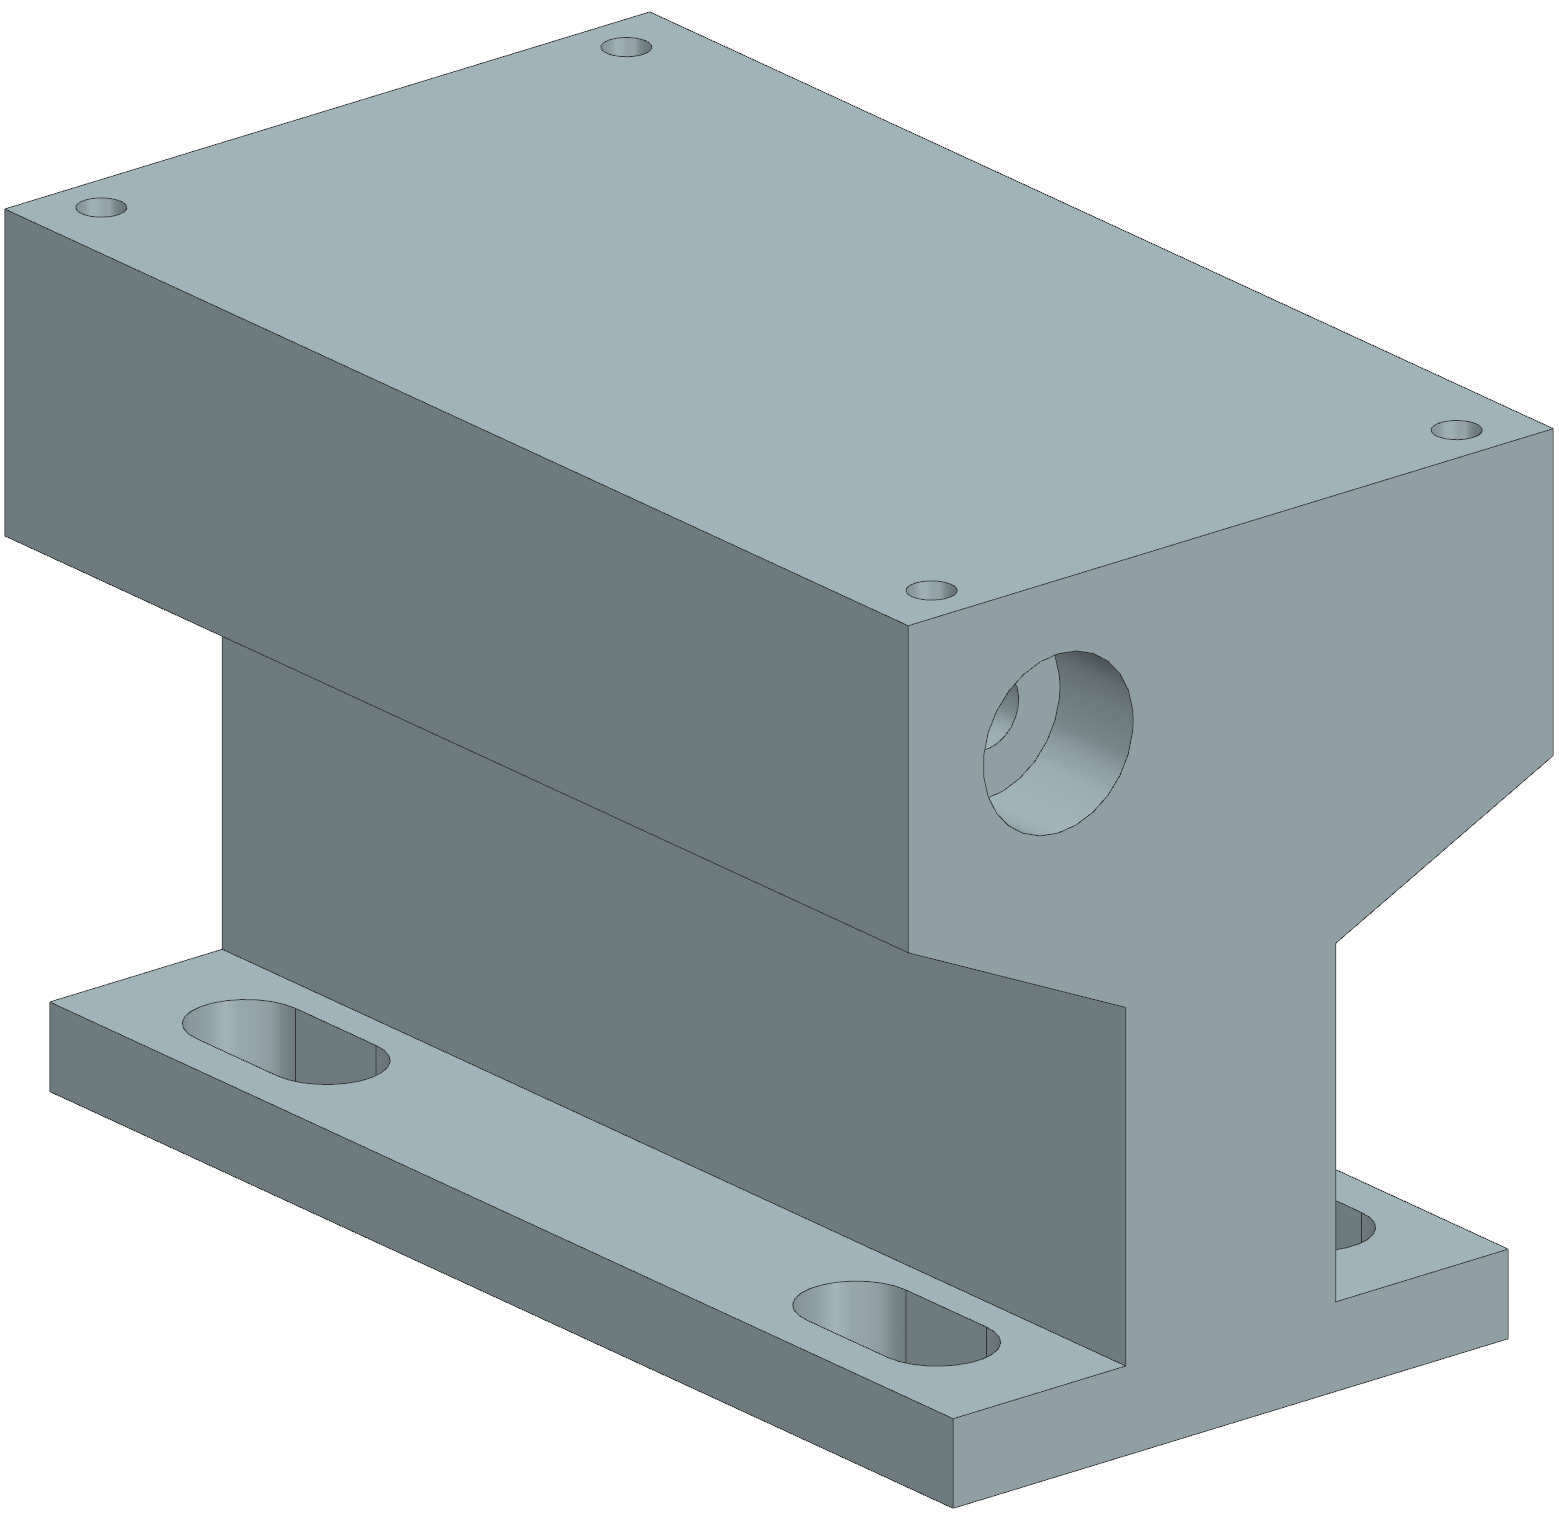
\includegraphics[scale=0.35]{98_images/kuehlblock_isometrie.PNG}
    \caption{Der gesamte Kühlblock.}
    \label{fig:enter-label}
\end{figure}

\begin{figure}[H]
    \centering
    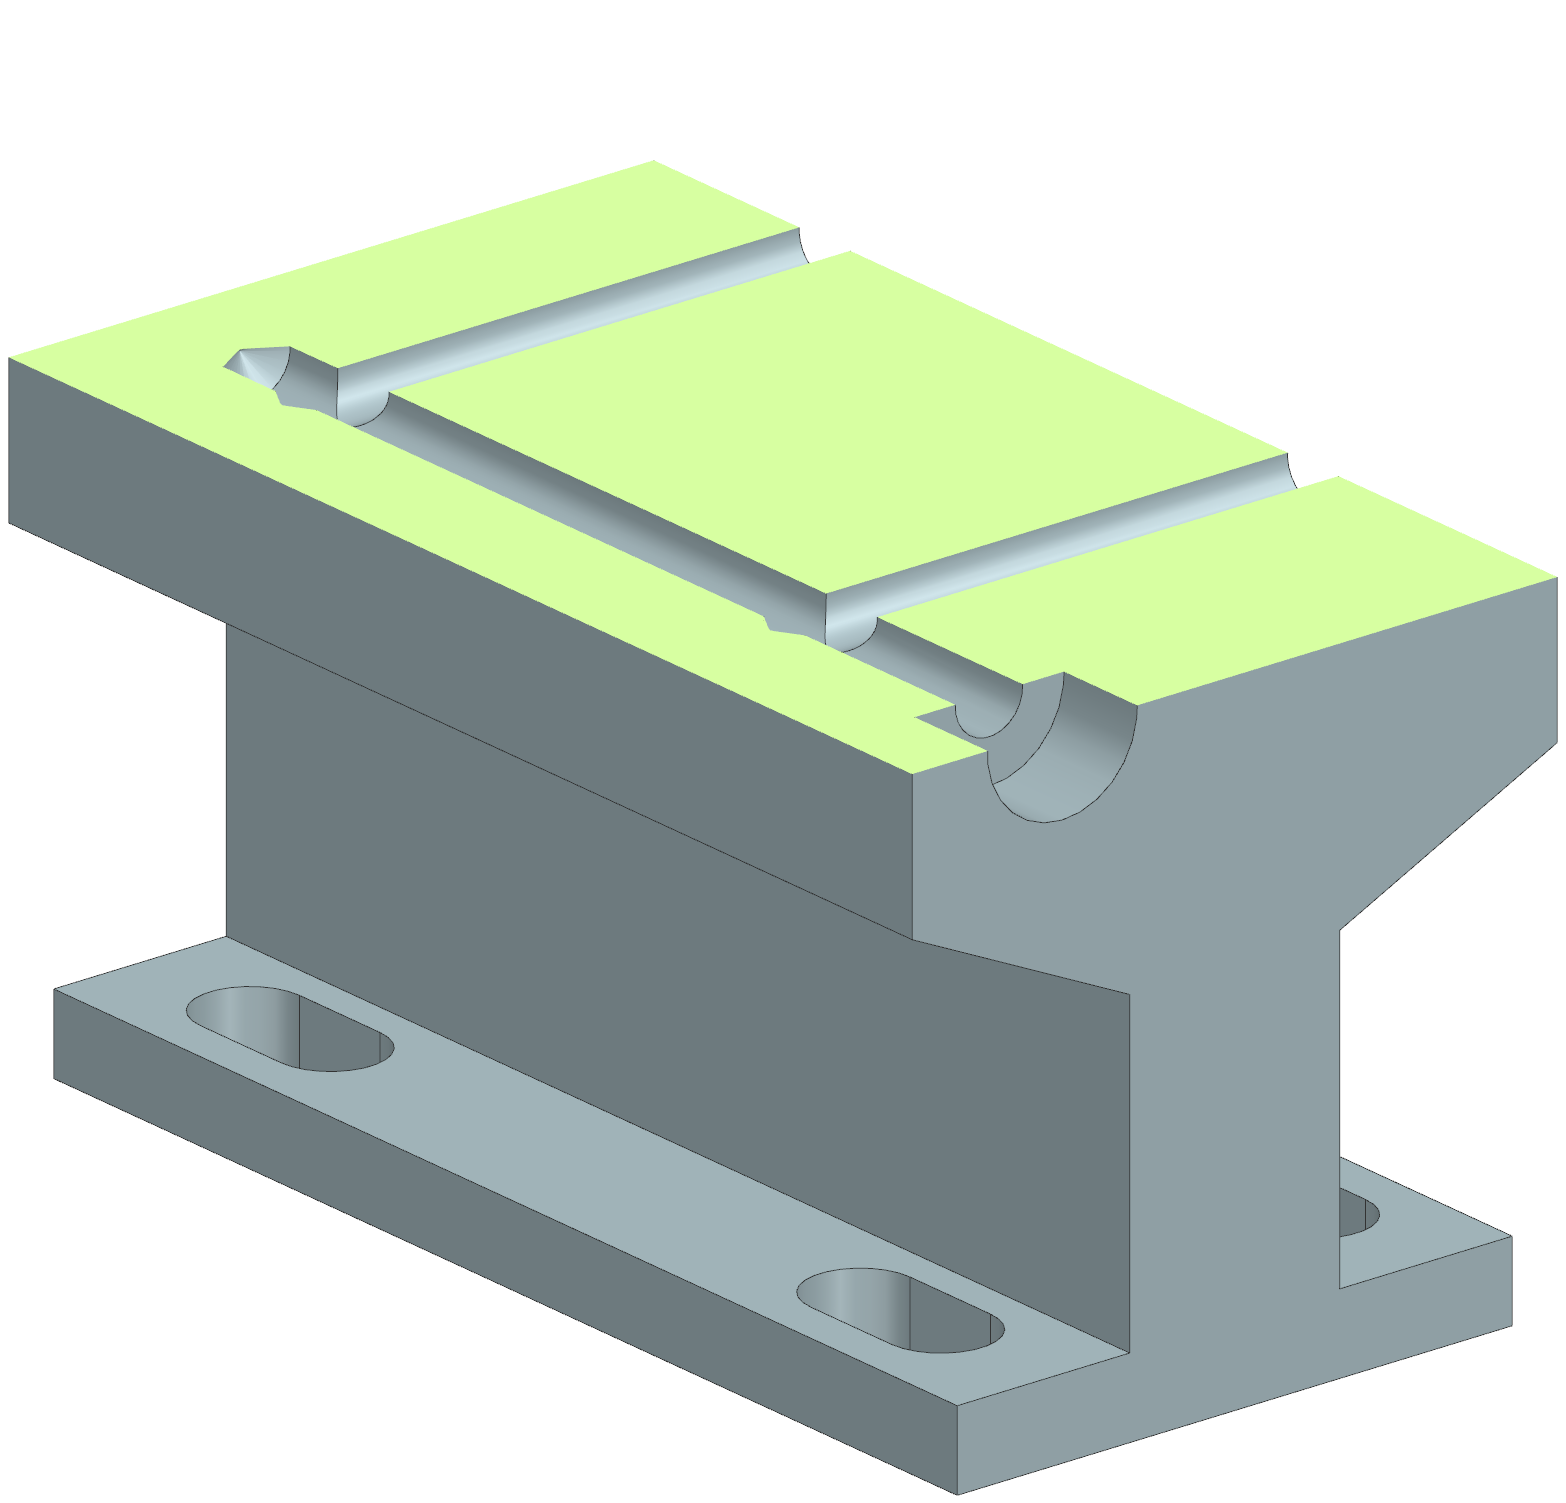
\includegraphics[scale=0.35]{98_images/kuehlblock_section.PNG}
    \caption{Die Schnittansicht für die Kanäle der Wasserkühlung.}
    \label{fig:enter-label}
\end{figure}

\subsection{Elektrische Verbindungen der Steuerung}
% \subsection{Beschreibung einiger Drittanbieter-Bibliotheken für die Programmierung}

% \subsection{Queue}
% <<In computer science, a queue is a collection of entities that are maintained in a sequence and can be modified by the addition of entities at one end of the sequence and the removal of entities from the other end of the sequence.>> [] https://en.wikipedia.org/wiki/Queue_(abstract_data_type)
\label{section:_libraries_py}

% \subsection{Tests}
\section{Programmcode}
\lstdefinestyle{custompython}{
  belowcaptionskip=1\baselineskip,
  breaklines=true,
  frame=L,
  xleftmargin=\parindent,
  numbers=left,
  language=Python,
  showstringspaces=false,
  basicstyle=\footnotesize\ttfamily,
  keywordstyle=\bfseries\color{green!40!black},
  commentstyle=\itshape\color{purple!40!black},
  identifierstyle=\color{blue},
  stringstyle=\color{orange},
}

\lstinputlisting[caption=Der Haupt-Quell-Code der Steuerung; custom\_gui.py, style=custompython]{gui_custom.py}
\label{main_src}

\lstinputlisting[caption=Der Quell-Code für die Steuerung der SPS; ldd\_control\_ang.py, style=custompython]{ldd_control_ang.py}
\label{ldd_src}

\subsubsection{Python Bibliothek - \textit{pandas}}
<<\textit{pandas} ist eine Programmbibliothek für Python zur Verarbeitung, Analyse und Darstellung von Daten. Insbesondere enthält sie Datenstrukturen und Operatoren für den Zugriff auf numerische Tabellen und Zeitreihen. \textit{pandas} ist Freie Software, veröffentlicht unter der 3-Klausel-BSD-Lizenz. Der Name leitet sich von dem englischen Begriff panel data (Paneldaten) ab, einer ökonometrischen Bezeichnung für Datensätze, die Beobachtungen über mehrere Zeiträume für dieselbe Untersuchungseinheit enthalten.>> [10]

\subsubsection{Python Bibliothek - \textit{NumPy}}
<<\textit{NumPy} ist eine Programmbibliothek für die Programmiersprache Python, die eine einfache Handhabung von Vektoren, Matrizen oder generell großen mehrdimensionalen Arrays ermöglicht. Neben den Datenstrukturen bietet \textit{NumPy} auch effizient implementierte Funktionen für numerische Berechnungen an.>> [11]

\end{appendix}
